\chapter{Methodology}
%%WHAT Is inference3
\label{chap:methodology}
In this section a performance model, characterising the deployment of deep learning models for inference, is presented. To understand these characteristics, the underlying factors that affect it need to be understood first. Therefore we first describe the problem space before we can map the problem space on the performance model.


\section{Problem Space}
The inference performance of a deep learning model is mainly affected by three factors, the architecture of the model itself and the hardware environment where it gets deployed and the framework performing the operations of the model on the hardware environment.
These three aspect are covered in this section.


\subsection{Deep Learning}
%%Bisschen genauer was deep learning input output...
%Einfluss auf inference latency an memory?
This section gives a brief, but nowhere complete overview of the deep learning field. We will focus on the basic structures and intuition behind deep learning models, as a comprehensive analysis would go beyond the scope of this thesis.

Deep learning are a subclass of neural networks.
The intention of a neural network is to make a prediction $\mathbf{\Hat{Y}}$ given an input $\mathbf{X}$ that is as close as possible to the underlying ground truth $\mathbf{Y}$. 
The difference of neural networks and deep learning networks is the amount of layers and hidden units. Deep learning models are built of many hidden layers and hidden units leading to deep architectures.
These deep architectures with often millions of parameters lead to a significant increase in computational power for both training and inference.
%While for simple linear regression model with a single variable a single computation
% ground through Y and the net predictions Y hat
\begin{figure}[!htb]
%%bild mit simpler architecture? Bild->conv->pool->flatten->dense-> output
    \centering
    \resizebox{.8\linewidth}{!}{\def\layersep{2.5cm}
\begin{tikzpicture}[shorten >=1pt,->,draw=black!50, node distance=\layersep]
    \tikzstyle{every pin edge}=[<-,shorten <=1pt]
    \tikzstyle{neuron}=[circle,fill=black!25,minimum size=17pt,inner sep=0pt]
    \tikzstyle{input neuron}=[neuron, fill=gray!50];
    \tikzstyle{output neuron}=[neuron, fill=gray!50];
    \tikzstyle{hidden neuron}=[neuron, fill=black!50];
    \tikzstyle{annot} = [text width=4em, text centered]

    % Draw the input layer nodes
    \foreach \name / \y in {1,...,4}
    % This is the same as writing \foreach \name / \y in {1/1,2/2,3/3,4/4}
        \node[input neuron, pin=left:$x_\y$] (I-\name) at (0,-\y) {};

    % Draw the hidden layer nodes
    \foreach \name / \y in {1,...,5}
        \path[yshift=0.5cm]
            node[hidden neuron] (H-\name) at (\layersep,-\y cm) {};
    % Draw the hidden layer nodes
    \foreach \name / \y in {2,...,4}
        \path[yshift=0.5cm]
            node[hidden neuron] (H2-\name) at (\layersep+2.5cm,-\y cm) {};
    % Draw the hidden layer nodes
    \foreach \name / \y in {1,...,5}
        \path[yshift=0.5cm]
            node[hidden neuron] (H3-\name) at (\layersep+5cm,-\y cm) {};
    % Draw the output layer node
    \node[output neuron,pin={[pin edge={->}]right:$\mathbf{\hat{Y}}$}, right of=H3-3] (O) {};

    % Connect every node in the input layer with every node in the
    % hidden layer.
    \foreach \source in {1,...,4}
        \foreach \dest in {1,...,5}
            \path (I-\source) edge (H-\dest);
            
    \foreach \source in {1,...,5}
        \foreach \dest in {2,...,4}
            \path (H-\source) edge (H2-\dest);
    \foreach \source in {2,...,4}
        \foreach \dest in {1,...,5}
            \path (H2-\source) edge (H3-\dest);

    % Connect every node in the hidden layer with the output layer
    \foreach \source in {1,...,5}
        \path (H3-\source) edge (O);

    % Annotate the layers
    \node[annot,above of=H-1, node distance=1cm] (hl) {Hidden layer};
    \node[annot,above of=H2-2, node distance=2cm] (hl2) {Hidden layer};
    \node[annot,above of=H3-1, node distance=1cm] (hl3) {Hidden layer};
    \node[annot,left of=hl] {Input layer};
    \node[annot,right of=hl3] {Output layer};
\end{tikzpicture}}
    \caption{Simple neural network}
    \label{fig:simpleNN}
\end{figure}

Figure \ref{fig:simpleNN} shows the structure of a simple neural network with input $\mathbf{X}$ and output $\mathbf{\Hat{Y}}$, where $\mathbf{X}$ is a vector of size four, meaning the neural network takes four features as its inputs. 
The output $\mathbf{\Hat{Y}}$ for this example is vector of only size one, hence the network predictions one value.
Between the input and output lay three fully connected hidden layers with five, three and again five hidden units.
Each of these hidden layers has a weight matrix $\mathbf{W\in\mathbb{R}^{m\times n}}$, where $\mathbf{m}$ is the number of hidden units and $\mathbf{n}$ the number of hidden units in the previous layer.
This weight matrices are needed to compute the state of each hidden layer by calculated the weighted sum on all its inputs.
For example the state of the first hidden layer is calculated by multiplying $\mathbf{W_1X}$, where $\mathbf{W_1}$ is the weight matrix of layer one and $\mathbf{X}$ the output of the previous layer, in this case the input layer.
To calculate  $\mathbf{\Hat{Y}}$ in the output layer using $\mathbf{W_O}$ , all previous states need to calculated consecutively. 
This chain of calculations needed to get from input $\mathbf{X}$ to output $\mathbf{\Hat{Y}}$ is also called forward-propagation, because the values of the input vector get passed through all layers by multiplication.
For example \ref{fig:simpleNN} all computations can be seen in equation \ref{eq:1}, with the shapes of all input/output vectors and weight matrices depicted in equation \ref{eq:2}.

\begin{equation} \label{eq:1}
\begin{gathered}
\mathbf{\hat{Y}(X)} = \mathbf{W_O(W_3(W_2(W_1X)))}
\end{gathered}
\end{equation}


\begin{equation} \label{eq:2}
\begin{gathered}
\mathbf{X} = \begin{bmatrix}
           x_{1} \\
           x_{2} \\
           x_{3} \\
           x_{4}
         \end{bmatrix},
\mathbf{W_1} = \begin{bmatrix}
           w_{11} & w_{12}& w_{13}& w_{14}\\
           w_{21} & w_{22}& w_{23}& w_{24} \\
           w_{31} & w_{32}& w_{33}& w_{34} \\
           w_{41} & w_{42}& w_{43}& w_{44} \\
           w_{51} & w_{52}& w_{53}& w_{54} 
         \end{bmatrix},
\mathbf{W_2} = \begin{bmatrix}
           w_{11} & w_{12}& w_{13}& w_{14}& w_{15}\\
           w_{21} & w_{22}& w_{23}& w_{24}& w_{25} \\
           w_{31} & w_{32}& w_{33}& w_{34}& w_{35} 
         \end{bmatrix},\\ \\
\mathbf{W_3} = \begin{bmatrix}
           w_{11} & w_{12}& w_{13}\\
           w_{21} & w_{22}& w_{23} \\
           w_{31} & w_{32}& w_{33} \\
           w_{41} & w_{42}& w_{43} \\
           w_{51} & w_{52}& w_{53} 
         \end{bmatrix},
\mathbf{W_O} = \begin{bmatrix} w_{11} & w_{12}& w_{13}& w_{14}& w_{15} \end{bmatrix},
\mathbf{\hat{Y}} = \begin{bmatrix} y_1 \end{bmatrix}
%\hat{Y} = (1\times5)(5\times3)(3\times5)(5\times4) (4\times1) = (1\times5)(5\times3)(3\times5)(5\time1) = (1\times5)(5\times3)(3\times1) = (1\times5)(5\times1) = 1
\end{gathered}
\end{equation}

For sake of simplicity the example does not use activation functions $\mathbf{\sigma}$ (e.\,g. ReLU) and biases $\mathbf{b}$, which would usually be used in practice in the form of $\mathbf{\sigma(WX+b)}$ instead of $\mathbf{WX}$.
Activation functions are needed to decide if a neuron (hidden unit) fires or not as well as minimising the risk of exploding/vanishing gradients.
%beispielrechnung für das nn


This simple network only contains three hidden layers with at most five hidden layers and thus 45 parameters, but in practice state of the art deep learning models contain often millions of parameters. 
The forward propagation of such models often need more than one GFLOPS, leading to high computational demands for real-time AI applications.

%15+5+15+20 = 45 parameters
%large network >10 000 000 param

There are many different operators and network architectures, all with different computational demands, thus making performance prediction very complex.
Since we will use image classification as a use case for the experimentation, we will now present the basics of Convolutional Neural Networks, which are used for this use case.

\paragraph{Convolutional Neural Network}
This specific class of neural network achieved wide success in the field of image classification and detection in images. Convolutional Neural Networks (CNN) are used to extract features like complex shapes or colour patterns from images to perform image classification. 
%Abschnitt über convolutions und pooling?

Image classification network classify the contents of a image by outputting a class for the image with a respective confidence level, for example how likely an animal on a picture represents a cat.
A simple architecture for this classification task can be seen in figure \ref{fig:simpleCNN}.
The network expects input images as a three dimensional tensor $h\times w\times c$, where $h$ and $w$ are the fixed height and width of the image and $c$ is the number of channels, which in most cases is $3$ for the RGB channels.
An image needs to be preprocessed to match these shape specifications before feeding it to the network.
The fundamental building blocks of CNNs are multiple convolution layers, which extract features from the images. The first convolutional extract simple features like edges from the image, while the later convolutional layers combine these simple features to complex shapes like rectangles.
To reduce the spatial dimension of the feature maps, outputted by the convolution, a popular layer type added to CNNs are pooling layers.
After extracting the features the resulting tensor get flattened to a one dimensional tensor before getting fed to one or more fully connected layers.
The last fully connected layer contains the output of the network, in this case confidence levels for predefined labels (e.\,g. $80$\% cat).  


\begin{figure}[!htb]
%%bild mit simpler architecture? Bild->conv->pool->flatten->dense-> output
    \centering
    \resizebox{.95\linewidth}{!}{

\tikzset{every picture/.style={line width=0.75pt}} %set default line width to 0.75pt        

\begin{tikzpicture}[x=0.75pt,y=0.75pt,yscale=-1,xscale=1]
%uncomment if require: \path (0,360.3333282470703); %set diagram left start at 0, and has height of 360.3333282470703

%Shape: Rectangle [id:dp05899425458959939] 
\draw  [color={rgb, 255:red, 160; green, 160; blue, 160 }  ,draw opacity=1 ][fill={rgb, 255:red, 160; green, 160; blue, 160 }  ,fill opacity=1 ][line width=1.5]  (760,203) -- (776.83,203) -- (776.83,213.33) -- (760,213.33) -- cycle ;
%Image [id:dp4912524236296907] 
\draw (66.08,133.08) node  {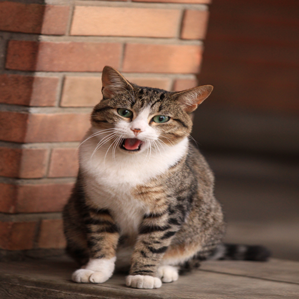
\includegraphics[width=79.62pt,height=79.62pt]{Bilder/European_cat_02_299.png}};
%Shape: Cube [id:dp48120440402395137] 
\draw  [fill={rgb, 255:red, 255; green, 255; blue, 255 }  ,fill opacity=1 ] (189,92.33) -- (149,52.33) -- (141,52.33) -- (141,171.33) -- (181,211.33) -- (189,211.33) -- cycle ; \draw   (141,52.33) -- (181,92.33) -- (189,92.33) ; \draw   (181,92.33) -- (181,211.33) ;
%Shape: Cube [id:dp1963658989292536] 
\draw  [fill={rgb, 255:red, 232; green, 232; blue, 232 }  ,fill opacity=1 ] (280,111.4) -- (241.94,73.33) -- (196,73.33) -- (196,170.27) -- (234.06,208.33) -- (280,208.33) -- cycle ; \draw   (196,73.33) -- (234.06,111.4) -- (280,111.4) ; \draw   (234.06,111.4) -- (234.06,208.33) ;
%Shape: Cube [id:dp9995029386851741] 
\draw  [fill={rgb, 255:red, 155; green, 155; blue, 155 }  ,fill opacity=1 ] (406,138.31) -- (377.08,109.4) -- (298,109.4) -- (298,171.48) -- (326.92,200.4) -- (406,200.4) -- cycle ; \draw   (298,109.4) -- (326.92,138.31) -- (406,138.31) ; \draw   (326.92,138.31) -- (326.92,200.4) ;
%Shape: Cube [id:dp47292096524654625] 
\draw  [fill={rgb, 255:red, 155; green, 155; blue, 155 }  ,fill opacity=1 ] (665.17,154.88) -- (648.62,138.33) -- (565,138.33) -- (565,173.85) -- (581.54,190.4) -- (665.17,190.4) -- cycle ; \draw   (565,138.33) -- (581.54,154.88) -- (665.17,154.88) ; \draw   (581.54,154.88) -- (581.54,190.4) ;
%Shape: Rectangle [id:dp9622310163181891] 
\draw   (736,94.33) -- (736,246.33) -- (717.17,246.33) -- (717.17,94.33) -- cycle ;
%Shape: Rectangle [id:dp3888373908322751] 
\draw   (778,104.33) -- (778,236.33) -- (759,236.33) -- (759,104.33) -- cycle ;
%Shape: Rectangle [id:dp6404657361959689] 
\draw  [fill={rgb, 255:red, 0; green, 0; blue, 0 }  ,fill opacity=1 ] (760,132) -- (776.83,132) -- (776.83,142.33) -- (760,142.33) -- cycle ;
%Straight Lines [id:da7775179037387632] 
\draw    (783.17,137.33) -- (806.17,137.33) ;
\draw [shift={(808.17,137.33)}, rotate = 180] [fill={rgb, 255:red, 0; green, 0; blue, 0 }  ][line width=0.75]  [draw opacity=0] (8.93,-4.29) -- (0,0) -- (8.93,4.29) -- cycle    ;

%Shape: Cube [id:dp25140851319063606] 
\draw  [fill={rgb, 255:red, 232; green, 232; blue, 232 }  ,fill opacity=1 ] (534.17,145.87) -- (510.63,122.33) -- (433,122.33) -- (433,172.86) -- (456.53,196.4) -- (534.17,196.4) -- cycle ; \draw   (433,122.33) -- (456.53,145.87) -- (534.17,145.87) ; \draw   (456.53,145.87) -- (456.53,196.4) ;
%Straight Lines [id:da07111443875380252] 
\draw    (189.17,135.33) -- (224.17,139.33) ;


%Straight Lines [id:da7555086779952114] 
\draw    (189.17,150.33) -- (224.17,139.33) ;


%Straight Lines [id:da6920716028952918] 
\draw    (190.17,124.33) -- (224.17,139.33) ;


%Straight Lines [id:da20921164719439567] 
\draw    (279.17,153.33) -- (314.17,157.33) ;


%Straight Lines [id:da5314884265558493] 
\draw    (279.17,168.33) -- (314.17,157.33) ;


%Straight Lines [id:da9607824424543641] 
\draw    (280.17,142.33) -- (314.17,157.33) ;


%Straight Lines [id:da22420538027937398] 
\draw    (405.17,162.33) -- (440.17,166.33) ;


%Straight Lines [id:da8064502796691653] 
\draw    (405.17,177.33) -- (440.17,166.33) ;


%Straight Lines [id:da9671090843658954] 
\draw    (406.17,151.33) -- (440.17,166.33) ;


%Straight Lines [id:da6406059045755481] 
\draw    (533.17,166.33) -- (568.17,170.33) ;


%Straight Lines [id:da9716418537016991] 
\draw    (533.17,181.33) -- (568.17,170.33) ;


%Straight Lines [id:da548327903780097] 
\draw    (534.17,155.33) -- (568.17,170.33) ;


%Straight Lines [id:da32303530471950226] 
\draw    (665.17,171.33) -- (715.17,171.33) ;
\draw [shift={(717.17,171.33)}, rotate = 180] [fill={rgb, 255:red, 0; green, 0; blue, 0 }  ][line width=0.75]  [draw opacity=0] (8.93,-4.29) -- (0,0) -- (8.93,4.29) -- cycle    ;

%Straight Lines [id:da4465574217797632] 
\draw    (735.17,171.33) -- (757.17,171.33) ;
\draw [shift={(759.17,171.33)}, rotate = 180] [fill={rgb, 255:red, 0; green, 0; blue, 0 }  ][line width=0.75]  [draw opacity=0] (8.93,-4.29) -- (0,0) -- (8.93,4.29) -- cycle    ;

%Straight Lines [id:da9780199762846196] 
\draw    (784.17,209.33) -- (807.17,209.33) ;
\draw [shift={(809.17,209.33)}, rotate = 180] [fill={rgb, 255:red, 0; green, 0; blue, 0 }  ][line width=0.75]  [draw opacity=0] (8.93,-4.29) -- (0,0) -- (8.93,4.29) -- cycle    ;


% Text Node
\draw (840,135) node  [align=left] {Cat \ $\displaystyle 0.8$};
% Text Node
\draw (185,219) node  [align=left] {$\displaystyle c$};
% Text Node
\draw (153,199) node [rotate=-45.72] [align=left] {$\displaystyle w$};
% Text Node
\draw (131,111) node [rotate=-269.52] [align=left] {$\displaystyle h$};
% Text Node
\draw (235,54) node  [align=left] {Convolution};
% Text Node
\draw (339,89) node  [align=left] {Pooling};
% Text Node
\draw (609,119) node  [align=left] {Pooling};
% Text Node
\draw (724,72) node  [align=left] {Dense};
% Text Node
\draw (770,86) node  [align=left] {Dense};
% Text Node
\draw (689,153) node  [align=left] {Flatten};
% Text Node
\draw (477,103) node  [align=left] {Convolution};
% Text Node
\draw (145,35) node  [align=left] {Input};
% Text Node
\draw (842,207) node  [align=left] {Dog \ $\displaystyle 0.1$};
% Text Node
\draw (70,192) node  [align=left] {{\scriptsize source: [SeL] }};


\end{tikzpicture}}
    \caption{Simple image classification CNN}
    \label{fig:simpleCNN}
\end{figure}

%Add calculation example
\subsubsection{Training}

After constructing the architecture of a model it can be trained to reach the highest accuracy.
Since most neural network are type of supervised learning, a training data set with ground truth labels $\mathbf{Y}$ is needed for the training.
This training is done with forward- and back-propagation, where one or more samples of the training set is forward propagated through the network until reaching the output layer. Afterwards the $Loss\mathbf{(Y,\Hat{Y})}$ can be calculated, which measures the difference between the prediction $\mathbf{\Hat{Y}}$ and the ground truth $\mathbf{Y}$.

To optimise the network, the loss needs to be minimised to a minimum, meaning that the different between prediction and ground truth is as small as possible and the accuracy as high as possible.
Since there is no closed form solution to find this minimum, neural network use gradient descent, specifically back-propagation, to minimise the loss in an iterative process.
Given the loss of the network, the gradients of all weights in the network can be computed and afterwards the weights can be updated using a learning rate in respect to the gradient and learning rate.

This process of forward- and back-propagation is repeated for all sample in the training data set multiple times until the minimum loss is reached and therefore the highest possible accuracy.

\subsubsection{Inference}
%only forward prop

After the model is trained it is ready to be deployed in a production environment, where it can serve its predictions to an application. This process of forward propagating the input through a neural network, performing all computational operations defined in the model resulting in an output/prediction, is called inference.

But since models often require the input to be of a certain shape and the input given by an application often does not match that shape, a preprocessing step is often needed before the actual inference can be performed.
This preprocessing and inference process can also be seen in figure \ref{fig:InfProcess}.
%%Add visualization of input here
%%die dann im deployment wieder aufgreifen
\begin{figure}[H]
\centering


\tikzset{every picture/.style={line width=0.75pt}} %set default line width to 0.75pt        

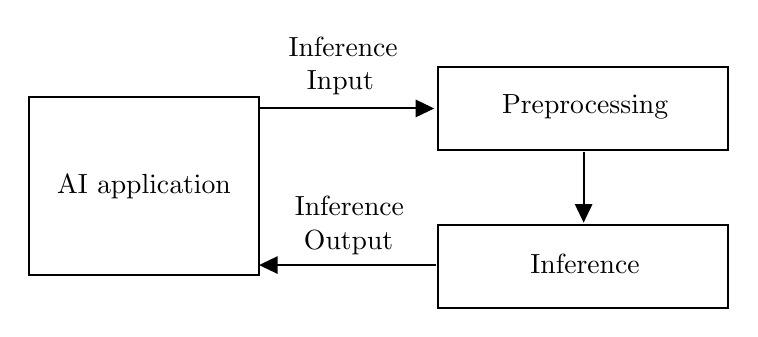
\begin{tikzpicture}[x=0.75pt,y=0.75pt,yscale=-1,xscale=1]
%uncomment if require: \path (0,300); %set diagram left start at 0, and has height of 300

%Shape: Rectangle [id:dp7725979857917211] 
\draw  [fill={rgb, 255:red, 255; green, 255; blue, 255 }  ,fill opacity=1 ] (262,80) -- (402,80) -- (402,120) -- (262,120) -- cycle ;
%Shape: Rectangle [id:dp3208391580840302] 
\draw  [fill={rgb, 255:red, 255; green, 255; blue, 255 }  ,fill opacity=1 ] (262,156) -- (402,156) -- (402,196) -- (262,196) -- cycle ;
%Straight Lines [id:da5532652572924177] 
\draw    (175.93,99.98) -- (258.29,99.98) ;
\draw [shift={(260.29,99.98)}, rotate = 180] [fill={rgb, 255:red, 0; green, 0; blue, 0 }  ][line width=0.75]  [draw opacity=0] (8.93,-4.29) -- (0,0) -- (8.93,4.29) -- cycle    ;

%Straight Lines [id:da9616587358279531] 
\draw    (332.29,121) -- (332.29,152.98) ;
\draw [shift={(332.29,154.98)}, rotate = 270] [fill={rgb, 255:red, 0; green, 0; blue, 0 }  ][line width=0.75]  [draw opacity=0] (8.93,-4.29) -- (0,0) -- (8.93,4.29) -- cycle    ;

%Straight Lines [id:da0888724954521467] 
\draw    (260.93,175.43) -- (177.93,175.43) ;
\draw [shift={(175.93,175.43)}, rotate = 360] [fill={rgb, 255:red, 0; green, 0; blue, 0 }  ][line width=0.75]  [draw opacity=0] (8.93,-4.29) -- (0,0) -- (8.93,4.29) -- cycle    ;

%Shape: Rectangle [id:dp6392688617606377] 
\draw  [fill={rgb, 255:red, 255; green, 255; blue, 255 }  ,fill opacity=1 ] (64.93,94.43) -- (175.93,94.43) -- (175.93,180.43) -- (64.93,180.43) -- cycle ;

% Text Node
\draw (333,99) node  [align=left] {Preprocessing};
% Text Node
\draw (333,175) node  [align=left] {Inference};
% Text Node
\draw (120.43,137.43) node  [align=left] {AI application};
% Text Node
\draw (216.43,79.43) node  [align=left] {Inference\\ \ \ Input};
% Text Node
\draw (219.43,156.43) node  [align=left] {Inference\\ \ Output};


\end{tikzpicture}
\caption{Visualisation of the inference process including preprocessing}
\label{fig:InfProcess}
\end{figure}
Note that the architecture of the inference model is often slightly different from the training model, as some operators are only needed for the training process and are thus removed for inference (e.\,g. dropout).






\subsubsection{Quantization}
\label{chap:quant}
Quantization is a technique that trades in model precision for better inference latencies, memory consumption during inference and model sizes.
Quantization describes the process of reducing the "precision representations of weights and, optionally, activations" \cite{tfLiteQuant} from floating point precision to for example 8-bit.
The weights/activations are either quantized after training the model with floats (Post Training Quantization) or the model is training with quantized weights/activations from the start (Quantization Aware Training). In the paper "Quantizing deep convolutional networks for
efficient inference"\cite{Quantizing} Krishnamoorthi performed a study on these technique with the following results:
8-bit quantization can lead to a model size reduction by a factor of 4, a 2-3x latency speedup on CPUs and DSPs, while reducing the model accuracies by 1\%.


\subsection{Deployment of Deep Learning Models}
Deep learning deployment describes the process of deploying a trained machine learning model to a production environment for inference purposes. 

%%Write more here
There can be differentiated in two different deployment methods, the first one is deploying the model directly to edge devices, while the second outsources the model to a cloud-backend, where the inference is performed and the prediction is sent back to the edge device.
\subsubsection{Edge Deployment}
Edge devices are characterised by offering a limited amount of hardware specifications such as amount of available energy, memory and overall computational power.
These devices are often mobile devices like smartphones, cars or Raspberry Pis.
Despite its limits, edge deployment also has some advantages, particular in reliability and security. 
For example in the case of image classification images are needed for the inference, which often contain sensible information and thus raise a data privacy/security concern.
Therefore edge deployment should be the preferred choice, if the inference performance is sufficient for the use case of real time AI applications.

In order to increase this performance various accelerators like better GPUs, TPUs or other dedicated neural network hardware components have been developed for edge devices.



\subsubsection{Cloud Deployment}
While the breakthroughs in deep learning are very interesting for AI applications on edge devices, the computational demand needed for edge deployment often exceeds the available power to be viable.
That is why the option of outsourcing the models to a cloud-backend has become a popular solution in the recent years.
Cloud-backends offer a huge amount of computational power, especially suitable for deep learning in the form of GPUs, TPUs, etc.


The big downside of cloud-based inference is the needed network connection, in particular for edge devices such as cars, where a reliable network connection can often not be guaranteed for example in rural areas. Hence this is not a viable solution for applications that are critical like autonomous driving.

While for the edge deployment necessary preprocessing steps are always done on the edge, for the case of cloud inference there a two possibilities. Either the input data is preprocessed to the correct shape before getting sent to the cloud-backend, or the input is sent unpreprocessed to the cloud. 
In the latter case the input gets preprocessed on the cloud. 
This can be justified by the same reasons as for the cloud inference, more computational power for intensive preprocessing.



\subsection{Deep Learning Inference Framework}
For both edge and cloud inference the underlying inference framework is important for the inference performance, since optimised kernels/operators or support of accelerators like GPUs can lead to significant performance improvements.
The framework needs to support the model operations as well as the hardware components to achieve a good performance.

%cloud inference network protocol

This is especially important for edge devices, where new accelerators are being developed at a fast pace.


%%
After analysing the problem space of deep learning inference for real-time AI applications on edge devices we can propose a performance model, that maps the aspects of the problem space on the performance.



\section{Performance Model}
All the aspects of hardware, model and the used inference framework have an impact on the performance, thus are the influencing factors of the performance model (see figure \ref{fig:perfmodel}). 
These inputs affect various performance metrics, of which inference latency and throughput are the most important ones for real-time AI applications on the edge. However, as the hardware on edge devices is limited and most of the times more than one application needs to run in parallel, low usages of the other depicted metrics are vital as well.
In the following we present performance metrics essential for the performance of real-time AI applications and the rationale behind them.
\begin{figure}[!htb]
\centering
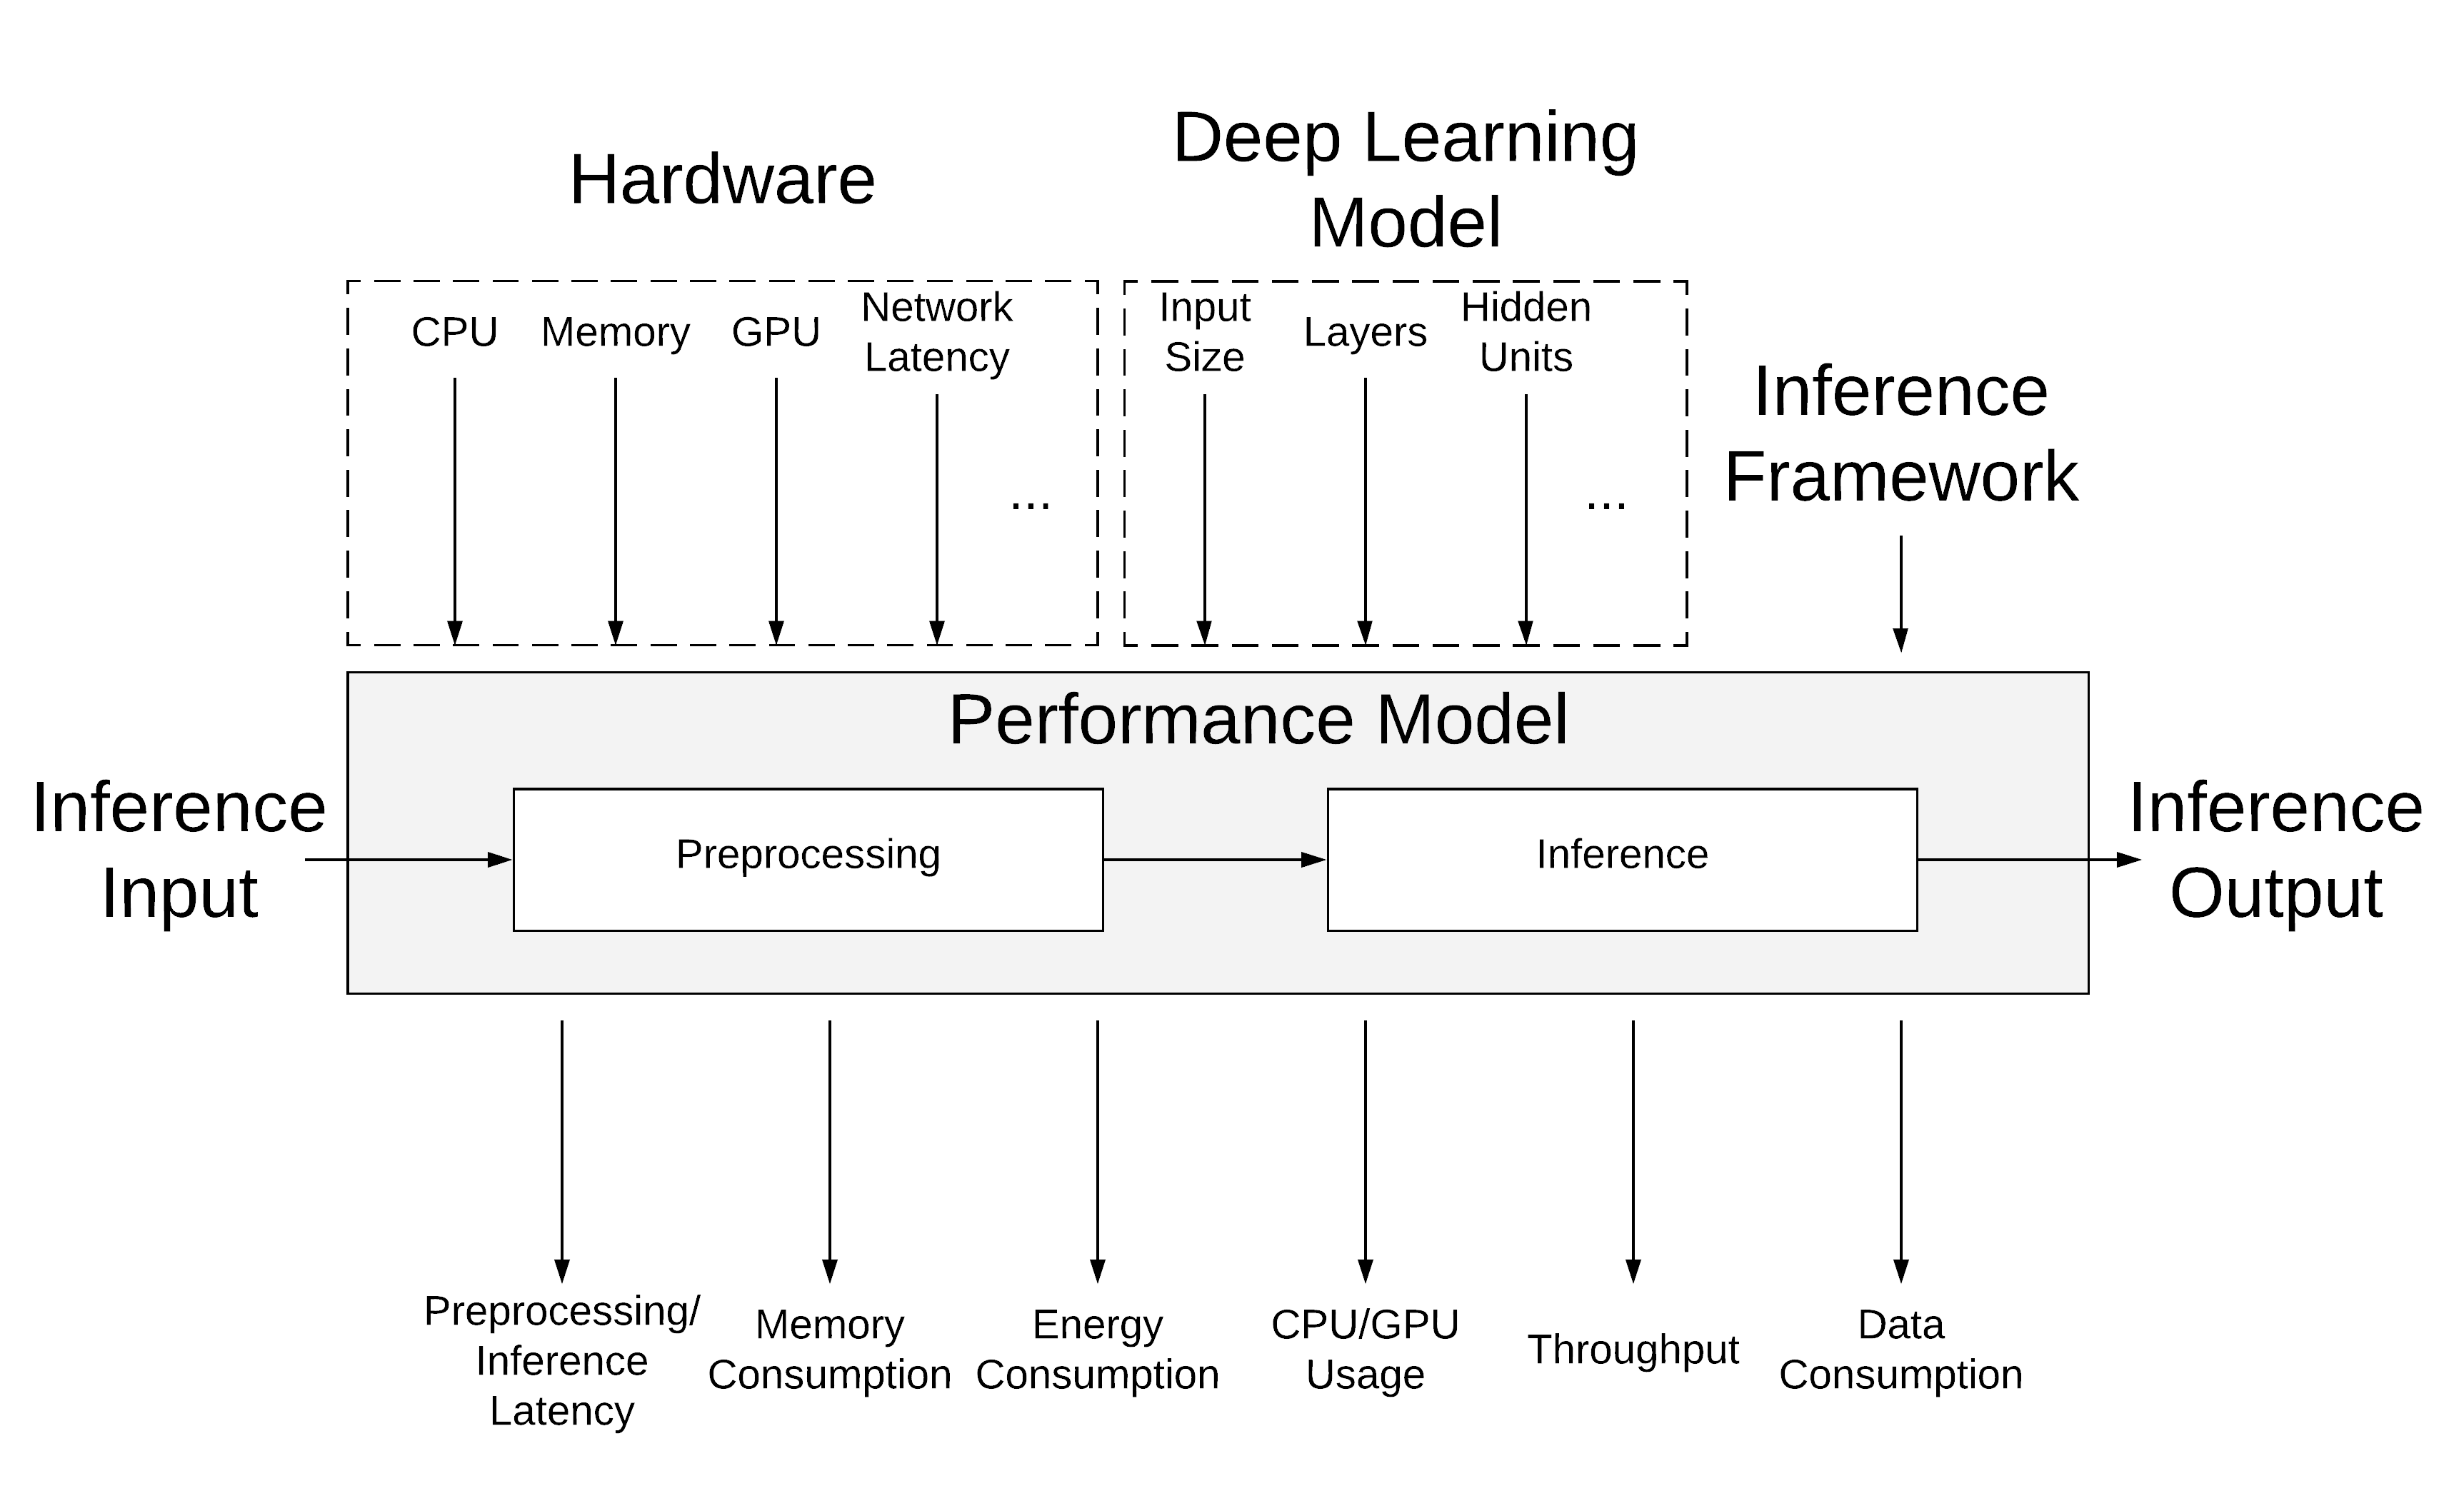
\includegraphics[width=0.99\textwidth]{./Bilder/trade_offs.png}
\caption{Performance Model}
\label{fig:perfmodel}
\end{figure}

Except the data consumption, which is only needed for cloud inference, because data is sent to a remote server, all metrics are relevant for both edge and cloud inference.
While accuracy is one of the most critical metrics for neural networks, it is only affected by the characteristics of the model and not by the deployment environment. Therefore we do not focus on accuracy in this thesis.

To get the model output for a given model input two steps are needed. The first one is the preprocessing step and transforms a given input into the format that is required by the deep learning model. Only then the actual inference operation can be performed to obtain the model output. Therefore the preprocessing takes a vital part in the general inference process and should be included in the performance model.

\subsection{Performance Metrics}
\label{chap:metrics}
Several metrics are important to measure the performance of the preprocessing and the inference steps. For the most of the following metrics we break down each metric into two sub-measurements, one for the preprocessing  and the other for the inference part.

Note that we only measure the impact on inference on the resources on the edge devices, not on the cloud-backend in case of cloud inference.
\subsubsection{Latency}
Latencies are a essential to determine the performance, since AI application often need predictions in realtime, resulting in the need of low latencies.
The time needed to transform the original input to a shape fit for feeding into the deep learning model is called $Latency_{preprocessing}$.
%%WALL CLOCK TIME ADD HERE
$Latency_{inference}$ describes the time needed from requesting a prediction from a deep learning model given an specific input until getting the prediction.
The latency needed to perform both preprocessing and inference for a given input is called $Latency_{total}$.
\subsubsection{Throughput}
In order to accomplish realtime AI a certain level of throughput is essential. Therefore the number of predictions per second is a valuable metric. 
Since preprocessing is a vital part of the inference process, the throughput impact caused by preprocessed is also of interest.

Therefore we differentiate between three types of throughput: $Throughput_{preprocessing}$, $Throughput_{inference}$ and $Throughput_{total}$.
$Throughput_{total}$ is the throughput of the preprocessing and inference latencies combined.



\subsubsection{Energy Consumption}
$Energy_{preprocessing}$ and $Energy_{inference}$, which describe the amount of energy consumed during preprocessing and inference, are particular important for mobile edge devices, since they often are powered by batteries with a limited lifespan. If the preprocessing or inference process consumes too much energy, the application using the model is not viable.


\subsubsection{CPU/GPU Usage}
Since the preprocessing/inference operations are most of the time not the only processes running on a system and other processes need to run simultaneously, the usages of CPU ($CPU_{inference}$, $CPU_{preprocessing}$) and GPU ($GPU_{inference}$, $GPU_{preprocessing}$) or other available accelerators are an important metric.
High usages would also indicate that performance would eventually be slowed down on devices with less CPU/GPU power.


\subsubsection{Memory Usage}
Similar to CPU usage, preprocessing and inference should not occupy the whole memory of the system or even demand more memory than the available memory. Therefore $Memory_{inference}$ and $Memory_{preprocessing}$ are of interest.
%\subsubsection{GPU Usage}
%If a GPU or an another accelerator is available their usage is of interest.

\subsubsection{Data Consumption}
$Data_{transmitted}$ and $Data_{received}$ are only relevant for cloud inference, as a request has to be sent to a remote server and the according response with prediction has to be sent back to the client. A high data consumption could slow down the inference latency significantly if the up- and downstream of the network connection is too slow. 

This is in particular important for the case where the input data for the model is preprocessed on the cloud, because the input data is often resized to a smaller shape during preprocessing. Therefore cloud preprocessing increased the amount of data that needs to be transmitted to the server. For slow network connections this could result in higher inference latencies.

%%Add table here?



%%%%%%%%%%%%%%%%%%%%%%%%%%
This section presented the factors influencing the performance of cloud and edge inference and the for the performance significant metrics.
To model the relation between these factors and metrics, we perform experiments on both edge and cloud inference using state of the art hardware, model and framework components. The setup and the result of these experiments are covered in the next section.
\endinput 